\title{คาบเรียนที่ 3: ฟังก์ชัน}
\frame{\titlepage}

\begin{frame}
\frametitle{เนื้อหาในคาบเรียนนี้}
\tableofcontents
\end{frame}

%%%%%%%%%%%%%%
\section{นิยามฟังก์ชัน}
\frame{\sectionpage}
%%%%%%%%%%%%%%

\begin{frame}
\addfig{0.8}{function_intro_price}{ความสัมพันธ์ระหว่างราคาป้าย และราคาที่ลดแล้ว}{}
\end{frame}

\begin{frame}
\frametitle{ความสัมพันธ์คืออะไร?}

\begin{defn}{}{}
ความสัมพันธ์ คือเซตของคู่อันดับ $(x,y)$
\end{defn}
\pa
เช่น 
\begin{itemize}
\item $R = \{(0,1), (1,2), (2,3)\}$
\item $S = \{(1,A), (1,B), (2,C), (A, D)\}$
\item $T = \{(\text{ปลา}, 3), (\text{กระจก}, 5), (\text{มด}, 2)\}$
\end{itemize}
\begin{slide}
แม้ว่าจะไม่มีเงื่อนไขว่าสมาชิกในคู่อันดับต้องเป็นอะไร แต่เราจะใช้ความสัมพันธ์ที่มีความหมาย เช่น $T$ คือความสัมพันธ์ระหว่างคำในภาษาไทย และจำนวนตัวอักษรในคำนั้น
\end{slide}
\end{frame}

\begin{frame}
\frametitle{แนวคิดแบบที่ 1}
มองเป็นเซต 2 เซต ที่มีลูกศรชี้จากตัวแปรต้น $x$ ในเซตหนึ่ง ไปยังตัวแปรตาม $f(x)$ อีกเซตหนึ่ง
\begin{figure}[h!]
\centering
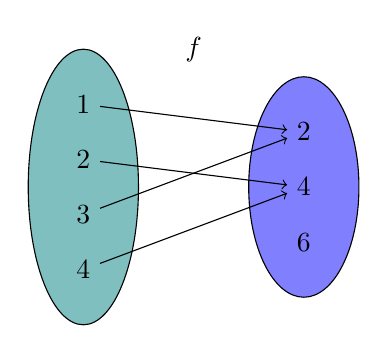
\begin{tikzpicture}[scale = 0.7]
\filldraw[fill = teal!50!white] (1,2.5) ellipse [x radius = 1, y radius = 2.5];
\filldraw[fill = blue!50!white] (5,2.5) ellipse [x radius = 1, y radius = 2];
\node at (1,4) (a1) {1};
\node at (1,3) (a2) {2};
\node at (1,2) (a3) {3};
\node at (1,1) (a4) {4};
\node at (5,3.5) (b1) {2};
\node at (5,2.5) (b2) {4};
\node at (5,1.5) (b3) {6};
\draw[->] (a1) -- (b1);
\draw[->] (a2) -- (b2);
\draw[->] (a3) -- (b1);
\draw[->] (a4) -- (b2);
\node at (3,5) {$f$};
\end{tikzpicture}
\caption{การมองฟังก์ชันเป็นความสัมพันธ์ของสมาชิกของเซต}
\end{figure}
\begin{slide}
ในตัวอย่างนี้ เราสร้างเป็นความสัมพันธ์ $R = \{(1,2), (2,4), (3,2), (4,4)\}$
\end{slide}
\end{frame}

\begin{frame}
\frametitle{แนวคิดแบบที่ 2}
มองเป็นตารางความสัมพันธ์ของข้อมูลสองชุด
\begin{table}[h!]
\setlength\arraystretch{1}
\centering
\begin{tabular}{|c|c|}
\hline
เดือน (ปี 2024) & จำนวนวัน \\
\hline
มกราคม & 31 \\
กุมภาพันธ์ & 29 \\
มีนาคม & 31 \\
เมษายน & 30 \\
พฤษภาคม & 31 \\
มิถุนายน & 30 \\
\hline
\end{tabular}
\caption{การมองฟังก์ชันเป็นตารางความสัมพันธ์ของข้อมูลสองชุด}
\end{table}
\begin{slide}
ในตัวอย่างนี้ เราสร้างเป็นความสัมพันธ์ $R = \{(\text{มกราคม},31), \ldots \}$
\end{slide}
\end{frame}

\begin{frame}
\frametitle{แนวคิดแบบที่ 3}
มองเป็นเครื่องจักร ที่รับตัวแปร $x$ เป็น input และให้ผลลัพธ์เป็น $y$
\begin{figure}[h!]
\centering
\begin{tikzpicture}
\draw[->] (-1,1) -- (0,1) node [left, pos=0] {รับค่า $x$};
\filldraw[fill = blue!50!white, draw=blue!50!black] (0,0) rectangle (3,2);
\node at (1.5,1) [scale = 2] {ฟังก์ชัน $f$};
\draw[->] (3,1) -- (4,1) node [right] {ส่งค่า $f(x)$};
\end{tikzpicture}
\caption{การมองฟังก์ชันเป็นเครื่องจักร}
\end{figure}
\end{frame}



\begin{frame}
\frametitle{แนวคิดแบบที่ 4}
สำหรับความสัมพันธ์จากเซตของจำนวนจริง $\mathbb{R}$ ไปยังเซตของจำนวนจริง $\mathbb{R}$
\begin{figure}[h!]
\centering
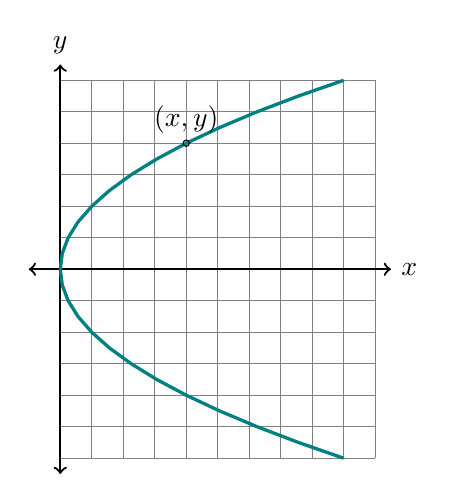
\begin{tikzpicture}[domain=-3:3, scale = 0.4]
\draw[help lines] (0,-6) grid (10,6);
\draw[<->, thick] (-1,0) -- (10.5,0) node[right] {$x$};
\draw[<->, thick] (0,-6.5) -- (0,6.5) node[above] {$y$};
\draw[color=teal, variable = \t, very thick] plot ({\t*\t},{\t*2});
\draw (4,4) circle [radius = 0.1cm] node[above] {$(x,y)$};
\end{tikzpicture}
\caption{กราฟของความสัมพันธ์}
\end{figure}
\end{frame}

\begin{frame}
\frametitle{ฟังก์ชันคืออะไร?}
\begin{defn}{}{}
ฟังก์ชัน คือ ความสัมพันธ์ที่ไม่มีสมาชิกตัวหน้าของสองคู่อันดับใดๆ เหมือนกัน \textbf{แต่สมาชิกตัวหลังต่างกัน} \pa
\medskip

เราเขียนแทนฟังก์ชันนี้ว่า 
\[f: A \rightarrow B\]
\pa อานว่า ``$f$ เป็นฟังก์ชันจาก $A$ ไป $B$''
\end{defn}
\pa
เราเขียนแทนฟังก์ชันในรูป
\[ y = f(x) \]
\pa โดยที่ $x$ เป็น \red{ตัวแปรอิสระ} (นั่นคือ input) \pa และ $y$ เป็น \green{ตัวแปรตาม} (นั่นคือ output) ที่ขึ้นอยู่กับ $x$
\end{frame}


\begin{frame}[t]
\begin{ex}
จงพิจารณาว่าความสัมพันธ์ต่อไปนี้เป็นฟังก์ชันหรือไม่
\begin{tasks}(1)
\task $R = \{(0,1), (1,2), (2,3)\}$
\task $S = \{(1,A), (1,B), (2,C), (A, D)\}$
\end{tasks}
\end{ex}
\begin{sol}
\begin{tasks}(1)
\task $R = \{(0,1), (1,2), (2,3)\}$ \pa เป็นฟังก์ชัน \pa เพราะไม่มีสมาชิกตัวหน้าของสองคู่อันดับใด ๆ ที่เหมือนกัน แต่สมาชิกตัวหลังต่างกัน
\task $S = \{\red{(1,A)}, \red{(1,B)}, (2,C), (A, D)\}$ \pa ไม่เป็นฟังก์ชัน \pa เพราะมีคู่อันดับ $(1,A)$ และ $(1,B)$ ที่สมาชิกตัวหน้าเหมือนกัน แต่สมาชิกตัวหลังต่างกัน
\end{tasks}
\end{sol}
\end{frame}

\begin{frame}
\frametitle{วิธีการตรวจสอบฟังก์ชัน}
1. ถ้าเขียนเป็นแผนภาพ สมาชิกในเซตแรก (ด้านซ้าย) ต้องมีลูกศรออกเพียง 1 เส้นเท่านั้น 


\begin{ex}
จงตรวจสอบว่าความสัมพันธ์ $R_1, R_2$ และ $R_3$ ต่อไปนี้เป็นฟังก์ชันหรือไม่

\begin{figure}[h!]
\centering
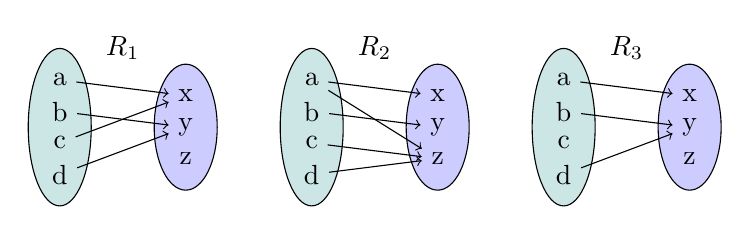
\begin{tikzpicture}[scale = 0.4]
\filldraw[fill = teal!20!white] (1,2.5) ellipse [x radius = 1, y radius = 2.5];
\filldraw[fill = blue!20!white] (5,2.5) ellipse [x radius = 1, y radius = 2];
\node at (1,4) (a1) {a};
\node at (1,3) (a2) {b};
\node at (1,2) (a3) {c};
\node at (1,1) (a4) {d};
\node at (5,3.5) (b1) {x};
\node at (5,2.5) (b2) {y};
\node at (5,1.5) (b3) {z};
\draw[->] (a1) -- (b1);
\draw[->] (a2) -- (b2);
\draw[->] (a3) -- (b1);
\draw[->] (a4) -- (b2);
\node at (3,5) {$R_1$};
\begin{scope}[xshift = 8cm]
\filldraw[fill = teal!20!white] (1,2.5) ellipse [x radius = 1, y radius = 2.5];
\filldraw[fill = blue!20!white] (5,2.5) ellipse [x radius = 1, y radius = 2];
\node at (1,4) (a1) {a};
\node at (1,3) (a2) {b};
\node at (1,2) (a3) {c};
\node at (1,1) (a4) {d};
\node at (5,3.5) (b1) {x};
\node at (5,2.5) (b2) {y};
\node at (5,1.5) (b3) {z};
\draw[->] (a1) -- (b1);
\draw[->] (a1) -- (b3);
\draw[->] (a2) -- (b2);
\draw[->] (a3) -- (b3);
\draw[->] (a4) -- (b3);
\node at (3,5) {$R_2$};
\end{scope}
\begin{scope}[xshift = 16cm]
\filldraw[fill = teal!20!white] (1,2.5) ellipse [x radius = 1, y radius = 2.5];
\filldraw[fill = blue!20!white] (5,2.5) ellipse [x radius = 1, y radius = 2];
\node at (1,4) (a1) {a};
\node at (1,3) (a2) {b};
\node at (1,2) (a3) {c};
\node at (1,1) (a4) {d};
\node at (5,3.5) (b1) {x};
\node at (5,2.5) (b2) {y};
\node at (5,1.5) (b3) {z};
\draw[->] (a1) -- (b1);
\draw[->] (a2) -- (b2);
\draw[->] (a4) -- (b2);
\node at (3,5) {$R_3$};
\end{scope}
\end{tikzpicture}
\caption{ภาพสำหรับตัวอย่างที่ \theexample}
\end{figure}
\end{ex}
\end{frame}

\begin{frame}
\begin{sol}
\begin{itemize}
\item $R_1$ เป็นฟังก์ชัน เนื่องจากสมาชิกในเซตแรกทุกตัวมีลูกศรออก 1 เส้นพอดี
\item $R_2$ ไม่เป็นฟังก์ชัน เนื่องจากมีลูกศรออกจาก $a$ ทั้งหมด 2 เส้น
\item $R_3$ ไม่เป็นฟังก์ชัน เนื่องจากไม่มีลูกศรออกจาก $c$ เลย
\end{itemize}

\begin{figure}[h!]
\centering
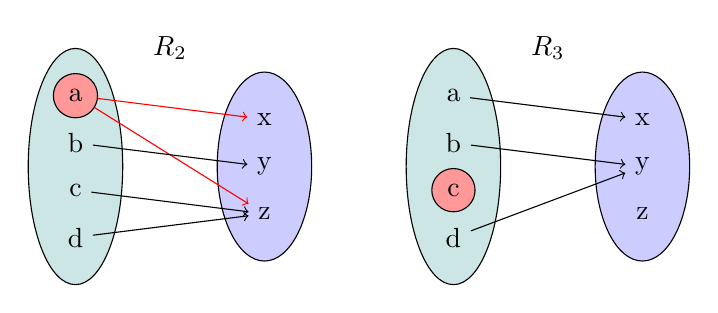
\begin{tikzpicture}[scale = 0.6]
\filldraw[fill = teal!20!white] (1,2.5) ellipse [x radius = 1, y radius = 2.5];
\filldraw[fill = blue!20!white] (5,2.5) ellipse [x radius = 1, y radius = 2];
\node[draw, circle, fill = red!40] at (1,4) (a1) {a};
\node at (1,3) (a2) {b};
\node at (1,2) (a3) {c};
\node at (1,1) (a4) {d};
\node at (5,3.5) (b1) {x};
\node at (5,2.5) (b2) {y};
\node at (5,1.5) (b3) {z};
\draw[->, red] (a1) -- (b1);
\draw[->, red] (a1) -- (b3);
\draw[->] (a2) -- (b2);
\draw[->] (a3) -- (b3);
\draw[->] (a4) -- (b3);
\node at (3,5) {$R_2$};
\begin{scope}[xshift = 8cm]
\filldraw[fill = teal!20!white] (1,2.5) ellipse [x radius = 1, y radius = 2.5];
\filldraw[fill = blue!20!white] (5,2.5) ellipse [x radius = 1, y radius = 2];
\node at (1,4) (a1) {a};
\node at (1,3) (a2) {b};
\node[draw, circle, fill = red!40] at (1,2) (a3) {c};
\node at (1,1) (a4) {d};
\node at (5,3.5) (b1) {x};
\node at (5,2.5) (b2) {y};
\node at (5,1.5) (b3) {z};
\draw[->] (a1) -- (b1);
\draw[->] (a2) -- (b2);
\draw[->] (a4) -- (b2);
\node at (3,5) {$R_3$};
\end{scope}
\end{tikzpicture}
\caption{ภาพสำหรับตัวอย่างที่ \theexample}
\end{figure}
\end{sol}
\end{frame}

\begin{frame}
\frametitle{วิธีการตรวจสอบฟังก์ชัน}
2. ถ้าเขียนเป็นกราฟ ให้ถือไม้บรรทัดตั้งขึ้น (นั่นคือ ขนานกับแกน $y$ และตั้งฉากกับแกน $x$) แล้วเลื่อนไม้บรรทัดขนานกับแกน $y$ ถ้าไม่มีส่วนไหนที่ตัดกับกราฟ 2 จุด จะนับว่าเป็นฟังก์ชัน

\begin{ex}
จงตรวจสอบว่ากราฟต่อไปนี้เป็นฟังก์ชันหรือไม่

\begin{figure}[h!]
\centering
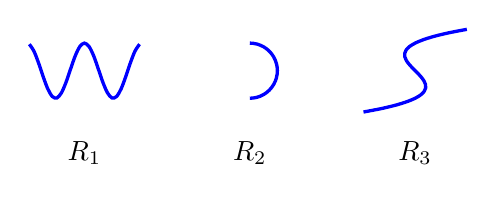
\begin{tikzpicture}[scale = 0.35, smooth]
\axes{-2}{2}{-2}{2};
\draw[blue, very thick, domain = -2:2] plot (\x, {cos(\x*3 r)});
\node at (0,-3) {$R_1$};
\begin{scope}[xshift = 6cm]
\axes{-2}{2}{-2}{2};
\draw[blue, variable = \t, very thick, domain = {-pi/2}:{pi/2}] plot ({cos(\t r)},{sin(\t r)});
\node at (0,-3) {$R_2$};
\end{scope}
\begin{scope}[xshift = 12cm]
\axes{-2}{2}{-2}{2};
\draw[blue, variable = \t, very thick, domain = -1.5:1.5] plot ({\t^3-\t},{\t});
\node at (0,-3) {$R_3$};
\end{scope}
\end{tikzpicture}
\caption{กราฟสำหรับตัวอย่าง \theexample}
\end{figure}

\end{ex}
\end{frame}

\begin{frame}
\begin{sol}
\begin{itemize}
\item $R_1$ เป็นฟังก์ชัน เนื่องจากไม่ว่าเราจะลากเส้นแนวตั้งที่ใด เส้นนั้นจะตัดกับกราฟไม่เกิน 1 จุดพอดี
\item $R_2$ ไม่เป็นฟังก์ชัน เนื่องจากมีเส้นแนวตั้งที่ลากแล้วตัดกับกราฟ 2 จุด
\item $R_3$ ไม่เป็นฟังก์ชัน เนื่องจากมีเส้นแนวตั้งที่ลากแล้วตัดกับกราฟ 2 จุด
\end{itemize}

\begin{figure}[h!]
\centering
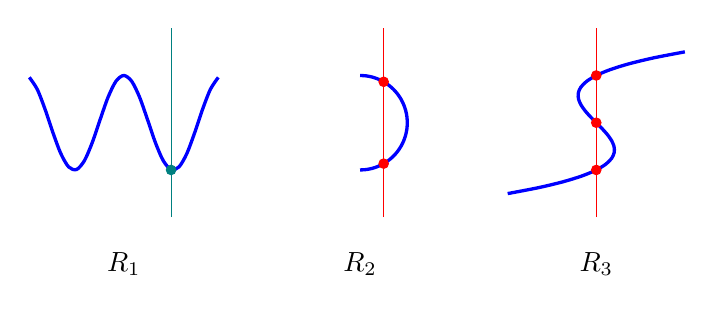
\begin{tikzpicture}[scale = 0.6, smooth]
\axes{-2}{2}{-2}{2};
\draw[color=blue, very thick, domain = -2:2] plot (\x, {cos(\x*3 r)});
\node at (0,-3) {$R_1$};
\draw[teal] (1,-2) --+ (0,4);
\filldraw[teal] (1,-1) circle [radius = 0.1cm];
\begin{scope}[xshift = 5cm]
\axes{-2}{2}{-2}{2};
\draw[color=blue, variable = \t, very thick, domain = {-pi/2}:{pi/2}] plot ({cos(\t r)},{sin(\t r)});
\node at (0,-3) {$R_2$};
\draw[red] (0.5,-2) --+ (0,4) ;
\filldraw[red] (0.5,{sqrt(3)/2}) circle [radius = 0.1cm];
\filldraw[red] (0.5,{-sqrt(3)/2}) circle [radius = 0.1cm];
\end{scope}
\begin{scope}[xshift = 10cm]
\axes{-2}{2}{-2}{2};
\draw[color=blue, variable = \t, very thick, domain = -1.5:1.5] plot ({\t^3-\t},{\t});
\node at (0,-3) {$R_3$};
\draw[red] (0,-2) --+ (0,4) ;
\filldraw[red] (0,-1) circle [radius = 0.1cm];
\filldraw[red] (0,0) circle [radius = 0.1cm];
\filldraw[red] (0,1) circle [radius = 0.1cm];
\end{scope}
\end{tikzpicture}
\caption{กราฟสำหรับตัวอย่าง \theexample}
\end{figure}
\end{sol}
\end{frame}

%%%%%%%%%%%%%%
\section{ประเภทของฟังก์ชัน}
\frame{\sectionpage}
%%%%%%%%%%%%%%

\begin{frame}
\frametitle{ประเภทของฟังก์ชัน}
1. ฟังก์ชันคงตัว (constant function) คือ ฟังก์ชันที่อยู่ในรูป 
\begin{block}{}
\[f(x) = c\]
 \end{block}
  เมื่อ $c$ เป็นจำนวนจริง ฟังก์ชันดังกล่าวจะมีกราฟเป็นเส้นตรงที่ขนานแกน x

\begin{figure}[h!]
\centering
\begin{tikzpicture}[scale = 0.5, smooth, domain = -2:2]
\axes{-2}{2}{-2}{2};
\draw[blue] plot (\x, 1.8);
\node[blue] at (0, -3) {$f(x) =4$};
\begin{scope}[xshift = 6cm]
\axes{-2}{2}{-2}{2};
\draw[red] plot (\x, 0.25);
\node[red] at (0,-3) {$f(x) = 0.5$};
\end{scope}
\begin{scope}[xshift = 12cm]
\axes{-2}{2}{-2}{2};
\draw[teal] plot (\x, -1);
\node[teal] at (0,-3) {$f(x) = -2$};
\end{scope}
\end{tikzpicture}
\caption{ตัวอย่างฟังก์ชันค่าคงตัว $f(x) = c$}
\end{figure}
\end{frame}

\begin{frame}
\frametitle{ประเภทของฟังก์ชัน}
2. ฟังก์ชันเชิงเส้น (linear function)  คือ ฟังก์ชันที่อยู่ในรูป 
\begin{block}{}
\[f(x) = ax+b\]
\end{block}
เมื่อ $a,b$ เป็นจำนวนจริง ฟังก์ชันดังกล่าวจะมีกราฟเป็นเส้นตรงไม่ขนานกับแกน  

\textbf{เช่น} $f(x) = 2x, f(x) = -3x + 1$  เป็นต้น \pa
\begin{figure}[h!]
\centering
\begin{tikzpicture}[scale = 0.5, smooth, domain = -2:2]
\axes{-2}{2}{-2}{2};
\draw[blue] plot (\x, {\x});
\node[blue] at (0,-3) {$f(x) =x$};
\begin{scope}[xshift = 6cm]
\axes{-2}{2}{-2}{2};
\draw[red] plot (\x, {1-\x});
\node[red] at (0,-3) {$f(x) = 1-x$};
\end{scope}
\begin{scope}[xshift = 12cm]
\axes{-2}{2}{-2}{2};
\draw[teal] plot[domain = -1:2] (\x, {2*\x-1});
\node[teal] at (0,-3) {$f(x) = 2x-1$};
\end{scope}
\end{tikzpicture}
\caption{ตัวอย่างฟังก์ชันเชิงเส้น $f(x) = ax+b$}
\end{figure}
\end{frame}

\begin{frame}
\frametitle{ประเภทของฟังก์ชัน}
3. ฟังก์ชันกำลังสอง (quadratic function) คือ ฟังก์ชันที่อยู่ในรูป  
\begin{block}{}
\[f(x) = ax^2+bx+c\]
\end{block}
เมื่อ $a,b,c$ เป็นจำนวนจริง และ $a \neq 0$ กราฟของฟังก์ชันกำลังสองคือส่วนโค้งที่อยู่ในรูปพาราโบลา และจะมีลักษณะหงายขึ้น หรือคว่ำลง

\begin{figure}[h!]
\centering
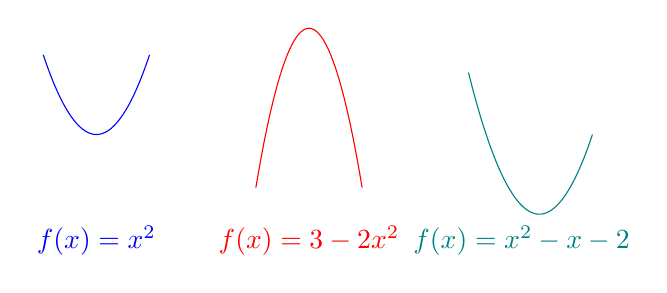
\begin{tikzpicture}[scale = 0.45, smooth, domain = -2:2]
\axes{-2}{2}{-2}{2};
\draw[blue] plot[domain = -1.5:1.5] (\x, {\x*\x});
\node[blue] at (0,-3) {$f(x) =x^2$};
\begin{scope}[xshift = 6cm]
\axes{-2}{2}{-2}{2};
\draw[red] plot[domain = -1.5:1.5] (\x, {3-2*(\x*\x)});
\node[red] at (0,-3) {$f(x) = 3-2x^2$};
\end{scope}
\begin{scope}[xshift = 12cm]
\axes{-2}{2}{-2}{2};
\draw[teal] plot[domain = -1.5:2] (\x, {(\x*\x)-\x-2});
\node[teal] at (0,-3) {$f(x) = x^2-x-2$};
\end{scope}
\end{tikzpicture}
\caption{ตัวอย่างฟังก์ชันเชิงกำลังสอง $f(x) = ax^2+bx+c$}
\end{figure}
\end{frame}

\begin{frame}
\frametitle{ประเภทของฟังก์ชัน}
4. ฟังก์ชันพหุนาม (polynomial function)  คือ ฟังก์ชันที่อยู่ในรูป 
\begin{block}{}
\[f(x) = a_n x^n + a_{n-1}x^{n-1} + \ldots + a_2 x^2 + a_1 x + a_0\]
\end{block}
โดยที่ $a_n, a_{n-1}, \ldots, a_2, a_1, a_0$ เป็นค่าคงตัว และ  $n \geq 0$ เป็นจำนวนเต็ม \pa

\begin{figure}[h!]
\centering
\begin{tikzpicture}[scale = 0.5, smooth, domain = -2:2]
\axes{-2}{2}{-2}{2};
\draw[blue] plot[domain = -1.2:1.2] (\x, {\x^3});
\node[blue, scale = 0.6] at (0,-3) {$f(x) =x^3$};
\begin{scope}[xshift = 6cm]
\axes{-2}{2}{-2}{2};
\draw[red] plot[domain = -2:2] (\x, {((\x*\x*\x*\x)-(5*(\x*\x))+4)/2});
\node[red, scale = 0.6] at (0,-3) {$f(x) = x^4-5x^2+4$};
\end{scope}
\begin{scope}[xshift = 12cm]
\axes{-2}{2}{-2}{2};
\draw[teal] plot[domain = -1.2:1.2] (\x, {(\x^6)+(\x^5)-(\x^4)-(\x^3)});
\node[teal, scale = 0.6] at (0,-3) {$f(x) = x^6+x^5-x^4-x^3$};
\end{scope}
\end{tikzpicture}
\caption{ตัวอย่างฟังก์ชันพหุนาม $f(x) = a_nx^n + a_{n-1}x^{n-1} + \cdots + a_1x + a_0$}
\end{figure}
\end{frame}

\begin{frame}
\frametitle{ประเภทของฟังก์ชัน}
5. ฟังก์ชันตรรกยะ (rational function)  คือ ฟังก์ชันที่อยู่ในรูป 
\begin{block}{}
\[f(x) = \frac{g(x)}{h(x)}\] 
\end{block}
โดยที่ $g(x)$  และ $h(x)$ เป็นฟังก์ชันพหุนาม และ $h(x)$ ไม่ใช่ฟังก์ชันคงตัว $h(x) = 0$ 

\begin{figure}[h!]
\centering
\begin{tikzpicture}[scale = 0.5, smooth, domain = -2:2]
\axes{-2}{2}{-2}{2};
\draw[blue] plot[domain = -2:-0.5] (\x, {1/\x});
\draw[blue] plot[domain = 0.5:2] (\x, {1/\x});
\node[blue, scale = 0.8] at (0,-3) {$f(x) = \frac{1}{x}$};
\begin{scope}[xshift = 6cm]
\axes{-2}{2}{-2}{2};
\draw[red] plot[domain = -2:2] (\x, {1/(\x*\x+1)});
\node[red, scale = 0.8] at (0,-3) {$f(x) = \frac{1}{x^2+1}$};
\end{scope}
\begin{scope}[xshift = 12cm]
\axes{-2}{2}{-2}{2};
\draw[teal] plot[domain = -2:-1.3] (\x, {(\x)/(\x*\x-1)});
\draw[teal] plot[domain = -0.8:0.8] (\x, {(\x)/(\x*\x-1)});
\draw[teal] plot[domain = 1.2:2] (\x, {(\x)/(\x*\x-1)});
\node[teal, scale = 0.8] at (0,-3) {$f(x) = \frac{x}{x^2-1}$};
\end{scope}
\end{tikzpicture}
\caption{ตัวอย่างฟังก์ชันตรรกยะ $f(x) = \tfrac{f(x)}{g(x)}$}
\end{figure}
\end{frame}

\begin{frame}
\frametitle{ประเภทของฟังก์ชัน}
6. ฟังก์ชันค่าสัมบูรณ์ (absolute value function)  คือ ฟังก์ชันที่มีเครื่องหมายค่าสัมบูรณ์ปรากฏอยู่

\begin{figure}[h!]
\centering
\begin{tikzpicture}[scale = 0.6, smooth, domain = -2:2]
\axes{-2}{2}{-2}{2};
\draw[blue] plot[domain = -2:2] (\x, {abs(\x)});
\node[blue, scale = 0.8] at (0,-3) {$f(x) = |x|$};
\begin{scope}[xshift = 6cm]
\axes{-2}{2}{-2}{2};
\draw[red] plot[domain = -2:2] (\x, {abs(2*\x-1)-2});
\node[red, scale = 0.8] at (0,-3) {$f(x) = |2x-1|-2$};
\end{scope}
\begin{scope}[xshift = 12cm]
\axes{-2}{2}{-2}{2};
\draw[teal] plot[domain = -2:2] (\x, {abs(1-\x*\x)});
\node[teal, scale = 0.8] at (0,-3) {$f(x) = |1-x^2|$};
\end{scope}
\end{tikzpicture}
\caption{ตัวอย่างฟังก์ชันค่าสัมบูรณ์}
\end{figure}
\end{frame}

\begin{frame}
\frametitle{ประเภทของฟังก์ชัน}
7.  ฟังก์ชันขั้นบันได (step function)  คือ ฟังก์ชันที่มีค่าคงตัวเป็นช่วงๆ ลักษณะกราฟของฟังก์ชันนี้เหมือนกับขั้นบันได เช่น 

\begin{figure}[h!]
\centering
\begin{tikzpicture}[scale = 0.6]
\axes{-2}{2}{-2}{2};
\draw[blue] (-2,-1) -- (0,-1) (0,1) -- (2,1) (0,-1) circle [radius = 0.1cm];
\filldraw (0,1) circle [radius = 0.1cm];
\node[blue, scale = 0.8] at (0,-3) {$f(x) = \begin{cases} -1; & x < 0 \\ 1;&x \geq 0\end{cases}$};
\begin{scope}[xshift = 6cm]
\axes{-2}{2}{-2}{2};
\draw[red] (-2,2) -- (-1,2) (-1,-1) -- (1,-1) (1,0) -- (2,0) (-1,2) circle [radius = 0.1cm] (1,0) circle [radius = 0.1cm];
\filldraw (-1,-1) circle [radius = 0.1cm] (1,-1) circle [radius = 0.1cm];
\node[red, scale = 0.8] at (0,-3) {$f(x) = \begin{cases} 2; & x < -1 \\ -1;&-1 \leq x \leq 1 \\ 0; & x > 1\end{cases}$};
\end{scope}
\begin{scope}[xshift = 12cm]
\axes{-2}{2}{-2}{2};
\foreach \x in {-2,-1,0,1}
{
	\draw [teal] (\x, \x) -- ({\x+1}, \x) circle [radius = 0.1cm];
	\filldraw[teal] (\x, \x) circle [radius = 0.1cm];
}
\node[teal, scale = 0.8] at (0,-3) {$f(x) = \lfloor x \rfloor$};
\end{scope}
\end{tikzpicture}
\caption{ตัวอย่างฟังก์ชันขั้นบันได}
\end{figure}
\end{frame}

%%%%%%%%%%%%%%
\section{โดเมนและเรนจ์}
\frame{\sectionpage}
%%%%%%%%%%%%%%

\begin{frame}
เรานิยามฟังก์ชันว่าเป็นความสัมพันธ์ระหว่างเซตสองเซต เราจะให้คำนิยามกับเซตทั้งสองที่เจาะจงขึ้น
\begin{defn}{}{}
\textbf{โดเมน (domain)} ของฟังก์ชัน $f$ (เขียนแทนด้วย $D_f$) คือเซตของค่า $x$ ทั้งหมดที่กำหนดไว้ (นั่นคือ $f(x)$ หาค่าได้)

\textbf{เรนจ์ (range) } ของฟังก์ชัน $f$ (เขียนแทนด้วย $R_f$) คือเซตของค่า $f(x)$ ทั้งหมดที่เป็นไปได้
\end{defn}
แต่ปกติแล้ว เราจะเขียนฟังก์ชันโดยไม่ระบุโดเมนชัดเจน ในกรณีนี้ให้นับว่าโดเมนคือเซตของค่า $x$ ทั้งหมดที่เป็นไปได้
\end{frame}

\begin{frame}
ถ้ากำหนดฟังก์ชันเป็นเซตของคู่อันดับ เราสามารถหาโดเมนและเรนจ์ได้จากคู่อันดับที่มีลูกศรชี้ออกหรือชี้เข้า

\begin{figure}[h!]
\centering
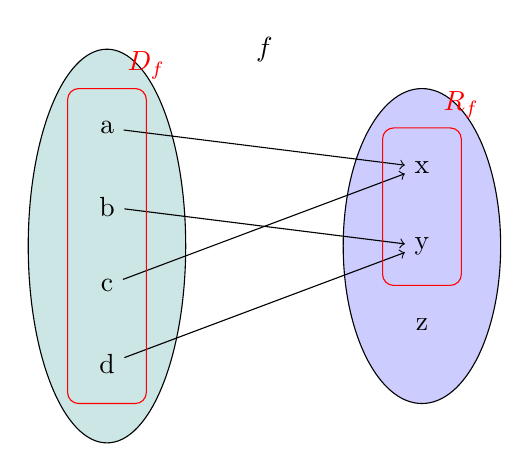
\begin{tikzpicture}
\filldraw[fill = teal!20!white] (1,2.5) ellipse [x radius = 1, y radius = 2.5];
\filldraw[fill = blue!20!white] (5,2.5) ellipse [x radius = 1, y radius = 2];
\node at (1,4) (a1) {a};
\node at (1,3) (a2) {b};
\node at (1,2) (a3) {c};
\node at (1,1) (a4) {d};
\node at (5,3.5) (b1) {x};
\node at (5,2.5) (b2) {y};
\node at (5,1.5) (b3) {z};
\draw[->] (a1) -- (b1);
\draw[->] (a2) -- (b2);
\draw[->] (a3) -- (b1);
\draw[->] (a4) -- (b2);
\node at (3, 5) {$f$};
\draw[rounded corners, red] (0.5, 0.5) rectangle (1.5, 4.5) node[above] {$D_f$};
\draw[rounded corners, red] (4.5, 2) rectangle (5.5, 4) node[above] {$R_f$};
\end{tikzpicture}
\caption{โดเมนและเรนจ์ของฟังก์ชัน $f$ คือเซต $D_f = \{a,b,c,d\}$ และ $R_f = \{x,y\}$}
\end{figure}
\end{frame}

\begin{frame}
ถ้ากำหนดฟังก์ชันเป็นกราฟ เราสามารถหาโดเมนได้โดยดูค่า $x$ ที่เป็นไปได้ทั้งหมดในกราฟ และหาเรนจ์ได้โดยดูค่า $y$ ที่เป็นไปได้ทั้งหมดในกราฟ

\begin{figure}[h!]
\centering
\begin{tikzpicture}
\axes{-2}{2}{-2}{2};
\draw[blue] plot[domain = -2:2] (\x, {abs(\x-1)-1});
\draw[red, |-|] (-2,-2.5) -- (2,-2.5) node[pos = 0.5, below] {$D_f$};
\draw[red, |-|] (-2.5,-1) -- (-2.5,2) node[pos = 0.5, left] {$R_f$};
\end{tikzpicture}
\caption{โดเมนและเรนจ์ของฟังก์ชัน $f$ จากการวิเคราะห์กราฟ}
\end{figure}
\end{frame}


\begin{frame}[t]
\begin{ex}
จงหาโดเมนและเรนจ์ของฟังก์ชัน $f(x) = x^2$
\end{ex}
\begin{sol}
สำหรับจำนวนจริง $x$ ใด ๆ เราทราบว่า $x^2$ หาค่าได้ \pa ฉะนั้นโดเมนของ $f$ คือเซตของจำนวนจริง \pa นั่นคือ $D_f = \mathbb{R}$ \pa

ส่วนค่า $y$ ทั้งหมดที่เป็นไปได้นั้น \pa คือจำนวนจริงบวกหรือศูนย์ \pa และถ้าให้ $y$ เป็นจำนวนจริงบวกหรือศูนย์แล้ว เราสามารถหาจำนวนจริง $\sqrt{y}$ \pa ที่ทำให้ $f(\sqrt{y}) = \sqrt{y}^2 = y$ \pa ฉะนั้นเรนจ์ของ $f$ คือ $R_f = [0 ,\infty)$
\end{sol}
\end{frame}


\begin{frame}[t]
\begin{ex}
จงหาโดเมนและเรนจ์ของฟังก์ชัน $f(x) = 2+\sqrt{3x-1}$
\end{ex}
\begin{sol}
เราทราบว่าตัวเลขในเครื่องหมายรากที่สองต้องเป็นบวกเสมอ \pa ฉะนั้น
\begin{eq*}
3x-1 &\geq& 0 \\ \pa
x &\geq& \frac{1}{3}
\end{eq*}
\pa นั่นคือ โดเมนของ $f$ คือเซต $D_f = [ \tfrac{1}{3}, \infty)$ ส่วนเรนจ์เราหาได้จากสมบัติของรากที่สองที่ว่า
\[\sqrt{3x-1} \geq 0\] 
\pa แล้วใช้สมบัติของอสมการเพื่อบวก 2 ทั้งสองข้าง ได้เป็น
\[2+\sqrt{3x-1} \geq 2\] 
\pa ฉะนั้นเรนจ์ของ $f$ คือเซต $R_f = [2,\infty)$
\end{sol}
\end{frame}

%%%%%%%%%%%%%%
\section[พีชคณิต]{พีชคณิตของฟังก์ชัน}
\frame{\sectionpage}
%%%%%%%%%%%%%%


\begin{frame}[t]
\frametitle{การหาค่าของฟังก์ชัน}
กำหนดให้ $f: A \rightarrow B$ \pa ถ้าเรามีค่า $a \in A$ แล้ว $f(a)$ คือค่าของฟังก์ชันได้ด้วยการแทนค่า $x=a$ ลงไปในฟังก์ชัน \pa โดยการเปลี่ยนตัวแปร $x$ \red{ทั้งหมด}ให้เป็นค่า $a$ \pa

\begin{ex}
กำหนดให้ $f(x) = 2x+1$ จงหา
\begin{tasks}(4)
\task $f(0)$
\task $f(1)$
\task $f(0.5)$ 
\task $f(100)$
\end{tasks}
\end{ex}
\begin{sol}
\begin{eqnarray*} 
\mbox{ถ้าให้ } x=0 &\mbox{ แล้ว }& \pa f(0) = 2(0) + 1 \pa = 1 \\ \pa
\mbox{ถ้าให้ } x=1 &\mbox{ แล้ว }& \pa f(1) = 2(1) + 1 \pa = 2+1 \pa = 3\\ \pa
\mbox{ถ้าให้ } x=0.5 &\mbox{ แล้ว }& \pa f(0.5) = 2(0.5) + 1 \pa = 1 + 1 \pa = 2\\ \pa
\mbox{ถ้าให้ } x=100 &\mbox{ แล้ว }& \pa f(100) = 2(100) + 1 \pa = 200 + 1 \pa = 201
\end{eqnarray*}
\end{sol}
\end{frame}


\begin{frame}[t]
\begin{ex}
กำหนดให้ $f(x) = x^2+x$ จงหา
\begin{tasks}(4)
\task $f(0)$
\task $f(2)$
\task $f(-3)$ 
\task $f\left(\frac{1}{3}\right)$
\end{tasks}
\end{ex}
\begin{sol}
\begin{tasks}(1)
\task $f(0) \pa = 0^2 + 0 = 0$ \pa
\task $f(2) \pa = 2^2 + 2 \pa= 4+2 \pa= 6$ \pa
\task $f(-3) \pa = (-3)^2 + (-3) \pa = 9 - 3 \pa = 6$ \pa
\task $f\left(\frac{1}{3}\right) \pa= \left(\frac{1}{3}\right)^2 + \frac{1}{3} \pa= \frac{1}{9} + \frac{1}{3} \pa= \frac{4}{9}$
\end{tasks}
\end{sol}
\end{frame}

\begin{frame}[t]
\frametitle{หมายเหตุ}
\begin{remark}{}
เราไม่จำเป็นต้องแทนค่า $x$ เป็นจำนวนจริงเท่านั้น แต่แทนเป็นตัวแปรอื่น หรือเป็นฟังก์ชันอื่นได้ด้วย
\pa
เช่น กำหนดให้ $f(x) = x^2+3x$ แล้ว
\begin{slide}
\begin{eqnarray*}
f(y) &=& y^2+3y \\ \pa
f(\Xi) &=& \Xi^2 + 3\Xi \\ \pa
f(x+5) &=& (x+5)^2 + 3(x+5) \\ \pa
f(x+h) &=& (x+h)^2 + 3(x+h) \\ \pa
f\left(\frac{1}{x}\right) &=& \left(\frac{1}{x}\right)^2 + 3\left(\frac{1}{x}\right) \pa
\end{eqnarray*}
\end{slide}
\end{remark}
\end{frame}

\begin{frame}
\frametitle{พีชคณิตของฟังก์ชัน}
พีชคณิตของฟังก์ชัน คือ การสร้างฟังก์ชันใหม่ โดยเอาฟังก์ชันเดิมอย่างน้อยสองฟังก์ชันมาบวก ลบ คูณ หรือหารกัน
\pa
\begin{prop}{}{}
ให้ $f$ และ $g$ เป็นฟังก์ชัน และ $c$ เป็นค่าคงตัว
\begin{enumerate}
\item $cf = \{(x,y) \mid y = cf(x)\}$ \pa
\item $f+g = \{(x,y) \mid y = f(x) + g(x) \}$ \pa
\item $f-g = \{(x,y) \mid y = f(x) - g(x) \}$ \pa
\item $fg = \{(x,y) \mid y = f(x)  g(x) \}$ \pa
\item $ \frac{f}{g} = \left\{(x,y) \mid y = \frac{f(x)}{g(x)} \right\}$ 
\end{enumerate}
\end{prop}
\end{frame}


\begin{frame}[t]
\begin{ex}
ให้ $f(x) = x+1$ และ $g(x) = 2x-3$ จงหา
\begin{tasks}(4)
\task $(2f)(x)$
\task $(f+g)(x)$ 
\task $(f - g)(x)$
\task $(3f + 2g)(x)$
\end{tasks}
\end{ex}
\begin{sol}
\begin{eqnarray*}
(2f)(x) \pa &=& 2f(x)  \\ \pa
&=& 2(x+1) \pa = 2x+2 \\ \pa
(f+g)(x) \pa &=& (x+1) + (2x-3)  \\ \pa
&=& (x+2x) + (1-3) \pa = 3x-2 \\ \pa
(f-g)(x) \pa &=& (x+1) - (2x-3) \\ \pa
&=& (x+1) + (-2x + 3) \pa = (x-2x) + (1+3) \pa = -x+4 \\ \pa
(3f + 2g) &=& 3f(x) + 2g(x) \\ \pa
&=& 3(x+1) + 2(2x-3) \pa = (3x+3) + (4x-6) \pa = (7x-3)
\end{eqnarray*}
\end{sol}
\end{frame}


\begin{frame}[t]
\begin{ex}
ให้ $f(x) = x+1$ และ $g(x) = 2x-3$ จงหา
\begin{tasks}(2)
\task $(fg)(x)$
\task $\left( \frac{f}{g} \right)(x)$
\end{tasks}
\end{ex}
\begin{sol}
\begin{eqnarray*}
(fg)(x) \pa &=& (x+1)(2x-3) \\ \pa
&=& 2x^2-3x+2x-3 \pa = 2x^2-x-3\\ \pa
\left(\frac{f}{g} \right)(x)&=& \frac{x+1}{2x-3}
\end{eqnarray*}
เราอาจต้องใช้การแยกตัวประกอบเพื่อทำให้เป็นรูปง่ายขึ้น หรืออาจใช้การหารพหุนามเพื่อลดเลขชี้กำลังลง เราได้ศึกษาเทคนิคเหล่านี้ในเรื่องพหุนามมาแล้ว และเราจะใช้แก้โจทย์ปัญหาในอนาคต
\end{sol}
\end{frame}


%%%%%%%%%%%%%%
\section{ฟังก์ชันประกอบ}
\frame{\sectionpage}
%%%%%%%%%%%%%%

\begin{frame}
\frametitle{ตัวอย่างที่ 1}
\addfig{0.8}{function_intro_factori}{การวางเครื่องจักรต่อเนื่อง \href{https://www.youtube.com/watch?v=v-tFGm9nCV0&ab_channel=StarGardenGames}{(Source)}}{}
\end{frame}

\begin{frame}
\frametitle{ตัวอย่างที่ 2}
กำหนดให้ราคาเริ่มต้นของสิ้นค้าคือ $x$ บาท
\medskip

ให้ฟังก์ชันราคาหลังจากคิดส่วนลดจากร้านค้า เป็น $f(x) = 0.5 x$
\medskip

ให้ฟังก์ชันราคาหลังจากคิดส่วนลดจากคูปอง เป็น $g(x) = 0.9 x$
\medskip

ถ้าเรานำส่วนลดที่ได้จากร้านค้า ไปใช้เป็นราคาในการคำนวณส่วนลดจากคูปอง จะได้ว่า
\begin{slide}
\[g(f(x) = g(0.5 x) = 0.9 (0.5 x) = 0.45 x \]

ซึ่งสังเกตว่า แทนที่จะคำนวณแยกกันสองรอบ เราสามารถคำนวณได้ทีเดียว โดยกำหนดฟังก์ชันใหม่คือ
\[ (g \circ f)(x) = 0.45 x\]
\end{slide}
\end{frame}

\begin{frame}
\frametitle{ฟังก์ชันประกอบ (composite function)}
นอกจากที่เราจะสามารถนำฟังก์ชันมาบวก ลบ คูณ หาร ได้ตามปกติแล้ว \pa เรายังสามารถนำมาประกอบกันเพื่อสร้างเป็นฟังก์ชันใหม่ได้ด้วย
\begin{defn}{}{}
 ฟังก์ชันประกอบ หรือ ฟังก์ชันคอมโพสิต ให้ $f(x)$ และ $g(x)$  เป็นฟังก์ชันใดๆ \pa ฟังก์ชันคอมโพสิท คือ $f \circ g$  โดยที่ 
 \[ (f \circ g)(x)= f(g(x))\]
\pa นั่นคือ เราแทนค่า $x$ เป็น $g(x)$ ในฟังก์ชัน $f(x)$
\end{defn}
\end{frame}

\begin{frame}
\begin{figure}[h!]
\centering
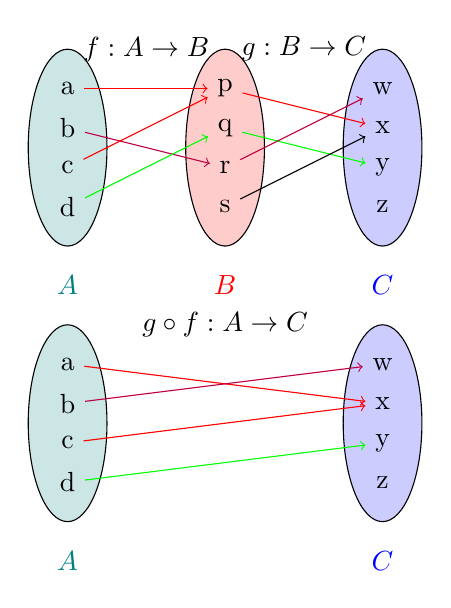
\begin{tikzpicture}[scale = 0.5]
\filldraw[fill = teal!20!white] (1,2.5) ellipse [x radius = 1, y radius = 2.5];
\node[teal] at (1,-1) {$A$};
\filldraw[fill = red!20!white] (5,2.5) ellipse [x radius = 1, y radius = 2.5];
\node[red] at (5,-1) {$B$};
\filldraw[fill = blue!20!white] (9,2.5) ellipse [x radius = 1, y radius = 2.5];
\node[blue] at (9,-1) {$C$};
\node at (1,4) (a1) {a};
\node at (1,3) (a2) {b};
\node at (1,2) (a3) {c};
\node at (1,1) (a4) {d};
\node at (5,4) (b1) {p};
\node at (5,3) (b2) {q};
\node at (5,2) (b3) {r};
\node at (5,1) (b4) {s};
\node at (9,4) (c1) {w};
\node at (9,3) (c2) {x};
\node at (9,2) (c3) {y};
\node at (9,1) (c4) {z};
\draw[->, red] (a1) -- (b1);
\draw[->, purple] (a2) -- (b3);
\draw[->, red] (a3) -- (b1);
\draw[->, green] (a4) -- (b2);
\draw[->, red] (b1) -- (c2);
\draw[->, green] (b2) -- (c3);
\draw[->, purple] (b3) -- (c1);
\draw[->] (b4) -- (c2);
\node at (3, 5) {$f: A \rightarrow B$};
\node at (7, 5) {$g: B \rightarrow C$};
\begin{scope}[yshift = -7cm]
\filldraw[fill = teal!20!white] (1,2.5) ellipse [x radius = 1, y radius = 2.5];
\node[teal] at (1,-1) {$A$};
\filldraw[fill = blue!20!white] (9,2.5) ellipse [x radius = 1, y radius = 2.5];
\node[blue] at (9,-1) {$C$};
\node at (1,4) (a1) {a};
\node at (1,3) (a2) {b};
\node at (1,2) (a3) {c};
\node at (1,1) (a4) {d};
\node at (9,4) (c1) {w};
\node at (9,3) (c2) {x};
\node at (9,2) (c3) {y};
\node at (9,1) (c4) {z};
\draw[->, red] (a1) -- (c2);
\draw[->, purple] (a2) -- (c1);
\draw[->, red] (a3) -- (c2);
\draw[->, green] (a4) -- (c3);
\node at (5, 5) {$g\circ f: A \rightarrow C$};
\end{scope}
\end{tikzpicture}
\caption{การสร้างฟังก์ชันประกอบ $g \circ f$ ในรูปแบบความสัมพันธ์}
\end{figure}
\end{frame}

\begin{frame}
\begin{figure}[h!]
\centering
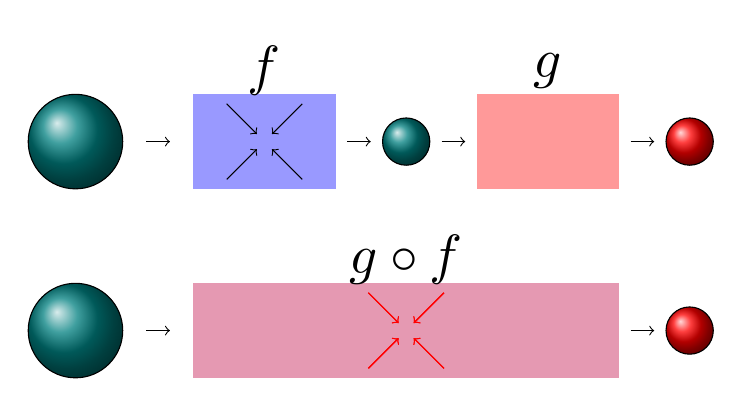
\begin{tikzpicture}[scale = 0.6]
\filldraw[blue!40] (0,0) rectangle (3,2);
\foreach \x in {-0.8,0.8}
{
	\foreach \y in {-0.8,0.8}
	{
		\draw[->] ({1.5+\x}, {1+\y}) -- ({1.5+(0.2*\x)},{1+(0.2*\y)});
	}
}
\filldraw[red!40] (6,0) rectangle (9,2);
\filldraw[ball color = teal] (-2.5,1) circle [radius = 1cm];
\filldraw[ball color = teal] (4.5,1) circle [radius = 0.5cm];
\filldraw[ball color = red] (10.5,1) circle [radius = 0.5cm];
\foreach \x in {-1, 3.25, 5.25, 9.25}
{
	\draw[->] (\x,1) -- ({\x+0.5},1);
}
\node[scale = 2] at (1.5, 2.5) {$f$};
\node[scale = 2] at (7.5, 2.5) {$g$};
\begin{scope}[yshift = -4cm]
\filldraw[purple!40] (0,0) rectangle (9,2);
\foreach \x in {-1,1}
\foreach \x in {-0.8,0.8}
{
	\foreach \y in {-0.8,0.8}
	{
		\draw[->, red] ({4.5+\x}, {1+\y}) -- ({4.5+(0.2*\x)},{1+(0.2*\y)});
	}
}
\filldraw[ball color = teal] (-2.5,1) circle [radius = 1cm];
\filldraw[ball color = red] (10.5,1) circle [radius = 0.5cm];
\foreach \x in {-1, 9.25}
{
	\draw[->] (\x,1) -- ({\x+0.5},1);
}
\node[scale = 2] at (4.5, 2.5) {$g \circ f$};
\end{scope}
\end{tikzpicture}
\caption{การสร้างฟังก์ชันประกอบในรูปของการทำงานเครื่องจักรแบบต่อเนื่อง}
\end{figure}
\end{frame}

\begin{frame}
\addfig{0.6}{function_composite_meme1}{ความแตกต่างระหว่าง $f \circ g$ และ $g \circ f$}{}
\end{frame}


\begin{frame}[t]
\begin{ex}
กำหนดให้ $f(x) = x+1$ และ $g(x) = x^2$ จงหา 
\begin{tasks}(2)
\task $(f \circ g)(x)$
\task $(g \circ f)(x)$
\task $(f \circ f)(x)$
\task $(g \circ g)(x)$
\end{tasks}
\end{ex}
\begin{sol}
\begin{eqnarray*}
(f \circ g)(x) \pa &=& f(\alert{g(x)}) \pa= \alert{g(x)} + 1 = x^2 + 1 \\ \pa
(g \circ f)(x) \pa &=& g(\green{f(x)}) \pa = \green{f(x)}^2 \pa = \green{(x+1)}^2
\end{eqnarray*}
\pa สังเกตว่า $(f \circ g)(x) \neq (g \circ f)(x)$ \pa นั่นคือลำดับการเขียนมีผลต่อผลลัพธ์
\begin{eqnarray*}
(f \circ f)(x) \pa &=& f(\green{f(x)}) \pa = \green{f(x)} + 1 \pa = \green{x+1} + 1 \pa = x+2 \\ \pa
(g \circ g)(x) \pa &=& g(\red{g(x)}) \pa = (\red{g(x)})^2 \pa = (\red{x^2})^2 \pa = x^4
\end{eqnarray*}
\end{sol}
\end{frame} 


\begin{frame}[t]
\begin{ex}
กำหนดให้ $f(x) = \sqrt{x} $ และ $g(x) = 2x+1$ จงหา 
\begin{tasks}(2)
\task $(f \circ g)(x)$
\task $(f \circ g)(4)$
\task $(g \circ f)(x)$
\task $(g \circ f)(4)$
\end{tasks}
\end{ex}
\begin{sol}
\begin{eqnarray*}
(f \circ g)(x) \pa &=& f(\alert{g(x)}) \pa= \sqrt{\alert{g(x)}} \pa = \sqrt{2x+1} \\ \pa
(f \circ g)(4) \pa &=& \sqrt{2(4) + 1 } \pa = \sqrt{9} \pa = 3 \\ \pa
(g \circ f)(x) \pa &=& g(\green{f(x)}) \pa = 2\green{f(x)}+1 \pa = 2\green{\sqrt{x}} + 1 \\ \pa
(g \circ f)(4) \pa &=& 2\sqrt{4} + 1 \pa =  2(2) + 1 \pa = 5
\end{eqnarray*}
\end{sol}
\end{frame}

%%%%%%%%%%%%%%
\section{ฟังก์ชันผกผัน}
\frame{\sectionpage}
%%%%%%%%%%%%%%

\begin{frame}
\frametitle{นิยามฟังก์ชันหนึ่งต่อหนึ่ง}
ก่อนจะนิยามฟังก์ชันผกผันได้ เราจะต้องนิยามฟังก์ชันหนึ่งต่อหนึ่งก่อน
\begin{defn}{}{}
$f: A \rightarrow B$ เป็นฟังก์ชันหนึ่งต่อหนึ่ง ก็ต่อเมื่อ ไม่มีคู่อันดับที่สมาชิกตัวหลังเหมือนกัน \textbf{แต่สมาชิกตัวหน้าต่างกัน}
\end{defn} \pa

เช่น $f = \{ (1,A), (2,B), (3,C)\}$ เป็นฟังก์ชัน 1 ต่อ 1 \pa

$g = \{(1,A), (2,A), (3,B)\}$ ไม่เป็นฟังก์ชัน 1 ต่อ 1 เพราะ $(1,A), (2,A)$ มีสมาชิกตัวหลังเหมือนกันแต่ตัวหน้าต่างกัน \pa
\end{frame}

\begin{frame}
\begin{figure}[h!]
\centering
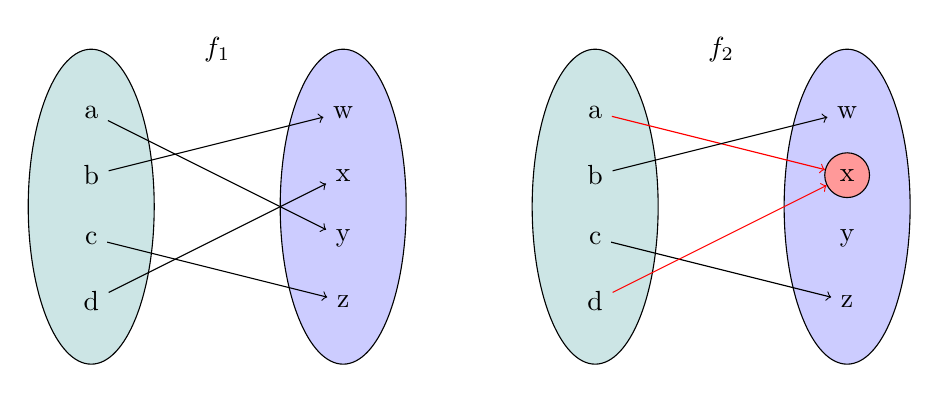
\begin{tikzpicture}[scale = 0.8]
\filldraw[fill = teal!20!white] (1,2.5) ellipse [x radius = 1, y radius = 2.5];
\filldraw[fill = blue!20!white] (5,2.5) ellipse [x radius = 1, y radius = 2.5];
\node at (1,4) (a1) {a};
\node at (1,3) (a2) {b};
\node at (1,2) (a3) {c};
\node at (1,1) (a4) {d};
\node at (5,4) (b1) {w};
\node at (5,3) (b2) {x};
\node at (5,2) (b3) {y};
\node at (5,1) (b4) {z};
\draw[->] (a1) -- (b3);
\draw[->] (a2) -- (b1);
\draw[->] (a3) -- (b4);
\draw[->] (a4) -- (b2);
\node at (3,5) {$f_1$};
\begin{scope}[xshift = 8cm]
\filldraw[fill = teal!20!white] (1,2.5) ellipse [x radius = 1, y radius = 2.5];
\filldraw[fill = blue!20!white] (5,2.5) ellipse [x radius = 1, y radius = 2.5];
\node at (1,4) (a1) {a};
\node at (1,3) (a2) {b};
\node at (1,2) (a3) {c};
\node at (1,1) (a4) {d};
\node at (5,4) (b1) {w};
\node[draw, circle, fill = red!40] at (5,3) (b2) {x};
\node at (5,2) (b3) {y};
\node at (5,1) (b4) {z};
\draw[->,red] (a1) -- (b2);
\draw[->] (a2) -- (b1);
\draw[->] (a3) -- (b4);
\draw[->,red] (a4) -- (b2);
\node at (3,5) {$f_2$};
\end{scope}
\end{tikzpicture}
\caption{ตัวอย่างฟังก์ชันหนึ่งต่อหนึ่ง $f_1$ และฟังก์ชันที่ไม่ใช่ฟังก์ชันหนึ่งต่อหนึ่ง $f_2$}
\end{figure}
\end{frame}

\begin{frame}
\frametitle{นิยามฟังก์ชันผกผัน}
\begin{defn}{}{}
กำหนดให้ $f$ เป็นฟังก์ชัน 1 ต่อ 1 \textbf{ ฟังก์ชันผกผันของ } $\mathbf{f}$ (เขียนแทนด้วย $f^{\, -1}$) คือฟังก์ชันที่มีสมบัติว่า
\[\text{ถ้า } y = f(x) \text{ แล้ว }f^{\, -1}(y) = x\]
\end{defn}
\end{frame}

\begin{frame}
ถ้ากำหนดฟังก์ชัน $f$ ในรูปแบบเซต เราสามารถสร้างฟังก์ชันผกผันได้ด้วยการสลับตำแหน่งเซต $A$ และ $B$ แล้วทำการสลับทิศทางลูกศรทั้งหมด

\begin{figure}[h!]
\centering
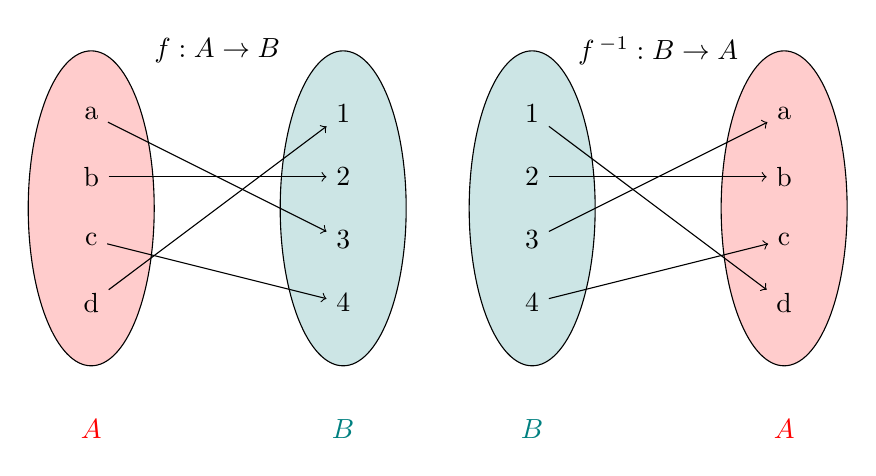
\begin{tikzpicture}[scale = 0.8]
\filldraw[fill = red!20!white] (1,2.5) ellipse [x radius = 1, y radius = 2.5];
\node[red] at (1,-1) {$A$};
\filldraw[fill = teal!20!white] (5,2.5) ellipse [x radius = 1, y radius = 2.5];
\node[teal] at (5,-1) {$B$};
\node at (1,4) (a1) {a};
\node at (1,3) (a2) {b};
\node at (1,2) (a3) {c};
\node at (1,1) (a4) {d};
\node at (5,4) (b1) {1};
\node at (5,3) (b2) {2};
\node at (5,2) (b3) {3};
\node at (5,1) (b4) {4};
\draw[->] (a1) -- (b3);
\draw[->] (a2) -- (b2);
\draw[->] (a3) -- (b4);
\draw[->] (a4) -- (b1);
\node at (3, 5) {$f: A \rightarrow B$};
\begin{scope}[xshift = 7cm]
\filldraw[fill = teal!20!white] (1,2.5) ellipse [x radius = 1, y radius = 2.5];
\node[teal] at (1,-1) {$B$};
\filldraw[fill = red!20!white] (5,2.5) ellipse [x radius = 1, y radius = 2.5];
\node[red] at (5,-1) {$A$};
\node at (5,4) (a1) {a};
\node at (5,3) (a2) {b};
\node at (5,2) (a3) {c};
\node at (5,1) (a4) {d};
\node at (1,4) (b1) {1};
\node at (1,3) (b2) {2};
\node at (1,2) (b3) {3};
\node at (1,1) (b4) {4};
\draw[<-] (a1) -- (b3);
\draw[<-] (a2) -- (b2);
\draw[<-] (a3) -- (b4);
\draw[<-] (a4) -- (b1);
\node at (3, 5) {$f\,^{-1}: B \rightarrow A$};
\end{scope}
\end{tikzpicture}
\caption{การสร้างฟังก์ชันผกผัน $f\,^{-1}$ ในรูปแบบความสัมพันธ์}
\end{figure}
\end{frame}

\begin{frame}
ถ้ากำหนดฟังก์ชัน $f$ ในรูปแบบการทำงานของเครื่องจักร เราสามารถสร้างฟังก์ชันผกผันได้ด้วยการหาว่าการทำงานแบบใดที่มีผลลัพธ์ตรงกันข้ามกับ $f$ เช่น ถ้า $f$ คือการลดขนาด แล้ว $f\,^{-1}$ คือการเพิ่มขนาด

\begin{figure}[h!]
\centering
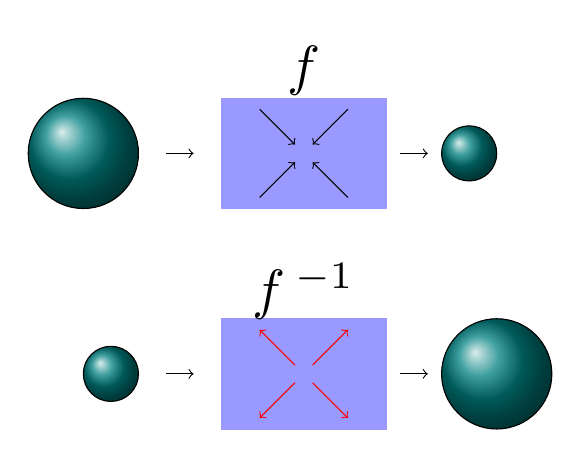
\begin{tikzpicture}[scale = 0.7]
\filldraw[blue!40] (0,0) rectangle (3,2);
\foreach \x in {-0.8,0.8}
{
	\foreach \y in {-0.8,0.8}
	{
		\draw[->] ({1.5+\x}, {1+\y}) -- ({1.5+(0.2*\x)},{1+(0.2*\y)});
	}
}
\filldraw[ball color = teal] (-2.5,1) circle [radius = 1cm];
\filldraw[ball color = teal] (4.5,1) circle [radius = 0.5cm];
\foreach \x in {-1, 3.25}
{
	\draw[->] (\x,1) -- ({\x+0.5},1);
}
\node[scale = 2] at (1.5, 2.5) {$f$};
\begin{scope}[yshift = -4cm]
\filldraw[blue!40] (0,0) rectangle (3,2);
\foreach \x in {-0.8,0.8}
{
	\foreach \y in {-0.8,0.8}
	{
		\draw[<-, red] ({1.5+\x}, {1+\y}) -- ({1.5+(0.2*\x)},{1+(0.2*\y)});
	}
}
\filldraw[ball color = teal] (-2,1) circle [radius = 0.5cm];
\filldraw[ball color = teal] (5,1) circle [radius = 1cm];
\foreach \x in {-1, 3.25}
{
	\draw[->] (\x,1) -- ({\x+0.5},1);
}
\node[scale = 2] at (1.5, 2.5) {$f\,^{-1}$};
\end{scope}
\end{tikzpicture}
\caption{การสร้างฟังก์ชันผกผัน $f\,^{-1}$ ในรูปการทำงานของเครื่องจักร}
\end{figure}
\end{frame}

\begin{frame}
ถ้ากำหนดฟังก์ชัน $f$ ในรูปแบบกราฟ เราสามารถสร้างฟังก์ชันผกผันได้ด้วยการแปลงจุด $(a,b)$ บนกราฟทั้งหมดให้กลายเป็นจุด $(b,a)$ ซึ่งมีค่าเท่ากับการสะท้อนกราฟฟังก์ชัน $y=f(x)$ บนเส้นแทยงมุม $y=x$ 

\begin{figure}[h!]
\centering
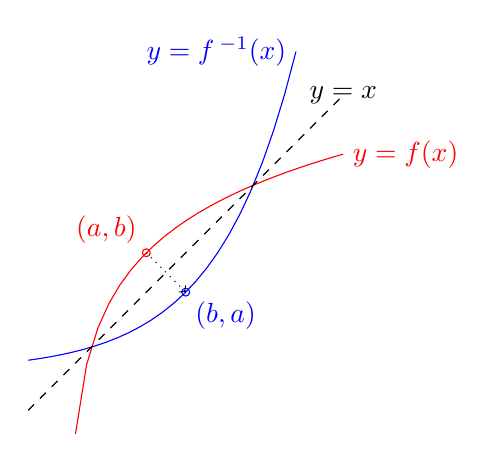
\begin{tikzpicture}
\axes{-2}{2}{-2}{2};
\draw[blue] plot[domain = -2:1.4] (\x, {exp(\x)-1.5}) node[left] {$y=f\,^{-1}(x)$};
\draw[red] plot[domain = -1.4:2] (\x, {ln(\x+1.5)}) node[right] 
{$y=f(x)$};
\draw[dashed] (-2,-2) -- (2,2) node {$y=x$};
\draw[red] (-0.5, 0) circle [radius = 0.05cm] node [above left] {$(a,b)$};
\draw[blue] (0, -0.5) circle [radius = 0.05cm] node [below right] {$(b,a)$};
\draw[dotted, ->] (-0.5,0) -- (0,-0.5);
\end{tikzpicture}
\caption{ตัวอย่างการหาฟังก์ชันผกผันจากกราฟ}
\end{figure}
\end{frame}

\begin{frame}
\addfig{0.6}{function_inverse_meme}{ภาพ meme เปรียบเทียบฟังก์ชันปกติ และฟังก์ชันผกผัน}{}
\end{frame}

\begin{frame}
\frametitle{วิธีหาฟังก์ชันผกผัน}
\begin{block}{}
\begin{enumerate}
\item กำหนดตัวแปร $y$ โดยที่ $y = f(x)$  \pa
\item สลับตัวแปรใหม่ ให้อยู่ในรูป $x = f(y)$ \pa
\item จัดรูปสมการให้ฝั่งซ้ายมี $y$ พจน์เดียว และฝั่งขวามีพจน์ $x$ และค่าคงตัวทั้งหมด \pa
\item สมการที่ได้จะอยู่ในรูป $y = f^{\, -1}$ ซึ่งเป็นฟังก์ชันผกผันที่ต้องการ
\end{enumerate}
\end{block}
\end{frame}


\begin{frame}[t]
\begin{ex}
กำหนดให้ $f(x) = x+2$ จงหา $f^{\, -1}(x)$
\end{ex}
\begin{sol}
\begin{itemize}
\item ขั้นแรกกำหนดตัวแปร $y = f(x)$ ขึ้นมาใหม่ \pa จะได้ 
\[y = x+2\] \pa
\item จากนั้นสลับตัวแปรใหม่จะได้เป็น \pa
\[x = y+2\] \pa
\item จัดรูปให้ $y$ อยู่ฝั่งซ้าย \pa จะได้
\[y = x-2\] \pa 
นั่นคือ $f^{-1}\,(x) = x-2$ เป็นฟังก์ชันผกผันที่ต้องการ
\end{itemize}
\end{sol}
\end{frame}


\begin{frame}[t]
\begin{ex}
กำหนดให้ $f(x) = x^2-3$ โดยที่ $x \geq 0$ จงหา $f^{\, -1}(x)$
\end{ex}
\begin{sol}
\begin{itemize}
\item ขั้นแรกกำหนดตัวแปร $y = f(x)$ ขึ้นมาใหม่ \pa จะได้ 
\[y = x^2-3, \text{ โดยที่ } x \geq 0\] \pa
\item สลับตัวแปรเป็น \pa
\[x = y^2-3, \text{ โดยที่ } y \geq 0\] \pa
จากนั้นจัดรูปใหม่\pa จะได้ 
\[y^2 = x+3  \qquad \rightarrow \qquad y = \pm \sqrt{x+3}\]
\pa แต่เนื่องจากเรากำหนดโดเมนที่มีค่า $y \geq 0$ \pa ฉะนั้นเราจึงได้ $y = \sqrt{x+3}$ \pa นั่นคือเราได้ฟังก์ชันผกผันเป็น  $f^{\, -1}(x) = \sqrt{x+3}$
\end{itemize}
\end{sol}
\end{frame}

\begin{frame}[t]
\frametitle{สมบัติของฟังก์ชันผกผัน}
\begin{prop}{}{}
กำหนดให้ $f: A \to B$ เป็นฟังก์ชันหนึ่งต่อหนึ่ง $D_f$ และ $R_f$ เป็นโดเมนและเรนจ์ของฟังก์ชันตามลำดับ
\begin{enumerate}
\item $f^{-1}: R_f \to A$ และเป็นฟังก์ชันหนึ่งต่อหนึ่งเช่นกัน
\item $(f \circ f^{-1}) (x) = x$ สำหรับทุก $x$ ใน $R_f$
\item $(f^{-1} \circ f)(x) = x$ สำหรับทุก $x$ ใน $A$
\end{enumerate}
\end{prop}
เช่น จากตัวอย่างก่อนหน้านี้เราทราบว่า $f(x) = x^2-3$ และ $f^{-1}(x) = \sqrt{x+3}$ ฉะนั้น
\begin{slide}
\[(f \circ f^{-1})(x) \pa = f( f^{-1}(x)) \pa = f( \sqrt{x+3} ) \pa = \sqrt{x+3}^2 - 3 \pa = (x+3) - 3 = x\]
\end{slide}
\end{frame}